%%%%%%%%%%%%%%%%%%%%%%%%%%%%%%%%%%%%%%%%%%%%%%%%%%%%%%%%%%
%
% Vzor pro sazbu kvalifikační práce
%
% Západočeská univerzita v Plzni
% Fakulta aplikovaných věd
% Katedra informatiky a výpočetní techniky
%
% Petr Lobaz, lobaz@kiv.zcu.cz, 2016/03/14
%
%%%%%%%%%%%%%%%%%%%%%%%%%%%%%%%%%%%%%%%%%%%%%%%%%%%%%%%%%%

% Možné jazyky práce: czech, english
% Možné typy práce: BP (bakalářská), DP (diplomová)
\documentclass[czech,DP]{thesiskiv}

% Definujte údaje pro vstupní strany
%
% Jméno a příjmení; kvůli textu prohlášení určete, 
% zda jde o mužské, nebo ženské jméno.
\author{Bc. František Koleňák}
\declarationmale

%alternativa: 
%\declarationfemale

% Název práce
\title{Klasifikace chyb SW \\na základě analýz z úložiště}

% 
% Texty abstraktů (anglicky, česky)
%
\abstracttexten{The text of the abstract (in English). It contains the English translation of the thesis title and a short description of the thesis.}

\abstracttextcz{Text abstraktu (česky). Obsahuje krátkou anotaci (cca 10 řádek) v češtině. Budete ji potřebovat i při vyplňování údajů o bakalářské práci ve STAGu. Český i anglický abstrakt by měly být na stejné stránce a měly by si obsahem co možná nejvíce odpovídat (samozřejmě není možný doslovný překlad!).
}

% Na titulní stranu a do textu prohlášení se automaticky vkládá 
% aktuální rok, resp. datum. Můžete je změnit:
%\titlepageyear{2016}
%\declarationdate{1. března 2016}

% Ve zvláštních případech je možné ovlivnit i ostatní texty:
%
%\university{Západočeská univerzita v Plzni}
%\faculty{Fakulta aplikovaných věd}
%\department{Katedra informatiky a výpočetní techniky}
%\subject{Bakalářská práce}
%\titlepagetown{Plzeň}
%\declarationtown{Plzni}

%%%%%%%%%%%%%%%%%%%%%%%%%%%%%%%%%%%%%%%%%%%%%%%%%%%%%%%%%%
%
% DODATEČNÉ BALÍČKY PRO SAZBU
% Jejich užívání či neužívání záleží na libovůli autora 
% práce
%
%%%%%%%%%%%%%%%%%%%%%%%%%%%%%%%%%%%%%%%%%%%%%%%%%%%%%%%%%%

% Zařadit literaturu do obsahu
\usepackage[nottoc,notlot,notlof]{tocbibind}

% Umožňuje vkládání obrázků
\usepackage[pdftex]{graphicx}

% Odkazy v PDF jsou aktivní; navíc se automaticky vkládá
% balíček 'url', který umožňuje např. dělení slov
% uvnitř URL
\usepackage[pdftex]{hyperref}
\hypersetup{colorlinks=true,
  unicode=true,
  linkcolor=black,
  citecolor=black,
  urlcolor=black,
  bookmarksopen=true}

% Při používání citačního stylu csplainnatkiv
% (odvozen z csplainnat, http://repo.or.cz/w/csplainnat.git)
% lze snadno modifikovat vzhled citací v textu
\usepackage[numbers,sort&compress]{natbib}

%%%%%%%%%%%%%%%%%%%%%%%%%%%%%%%%%%%%%%%%%%%%%%%%%%%%%%%%%%
%
% VLASTNÍ TEXT PRÁCE
%
%%%%%%%%%%%%%%%%%%%%%%%%%%%%%%%%%%%%%%%%%%%%%%%%%%%%%%%%%%
\begin{document}
%
\maketitle
\tableofcontents

\chapter{Úvod}
V souboru \texttt{literatura.bib} jsou uvedeny příklady, jak citovat knihu \cite{KnuthAOCP2}, článek v časopisu \cite{Hoare1961}, webovou stránku \cite{Graphics2D}.
 
\newpage

%Seznamte se s nástroji používanými pro řízení projektu a s daty která je možné z nich získat, zejména s důrazem na popisy opravovaných chyb a data která se k chybám váží.
\chapter{Řízení projektů}
Řízení projektu (někdy též projektové řízení) se zabývá řízením projektu, tedy časově ohraničené a ucelené sady činností a procesů, jejímž cílem je co nejefektivněji zavést, vytvořit nebo změnit něco konkrétního (definováno daným projektem).

Tradiční přístup řízení projektů je založen na důkladném naplánování na začátku projektu a řízení všech aktivit v průběhu projektu. Tento přístup (též známý jako vodopádový model) je nejvíce vhodný na projekty, které mají podobu cíle jasně danou a neměnnou (chodník, dům) a ve kterých je nutné dobře naplánovat všechny aktivity související s daným projektem. Tradiční přístup vyžaduje kvalitně popsaný cíl, výstupy a plán projektu.

Opakem tradičního přístupu je agilní přístup. Ten je založen na průběžném upřesňování cíle, díky interakci se zákazníkem či s uživateli výsledků projektu. Tento proces se označuje jako získávání zpětné vazby. Reagováním na vstupy od zákazníka je projekt dynamicky upravován a proto je vhodný na takové projekty, kde dochází k vývoji produktu, tedy tehdy když nelze předem kvalitně popsat a naplánovat vše do podrobností a bez zpětné vazby. Agilní přístup se často používá ve vývoji software.

\section{Fáze projektu}
Projekt se může nacházet v různých fázích (procesních skupinách). Tyto fáze se mohou lišit použitou metodou na řízení projektu, ale víceméně je struktura a podoba fází velice podobná. Nejčastějšími fázemi jsou:

\begin{itemize}
	\item {Zahájení} - Start projektu a vytyčení jeho mezí
	\item {Plánování} - Plánování částí projektu
	\item {Realizace} - Implementace rozplánované části
	\item {Monitorování a řízení} - Zpětná vazba od zákazníka, podpora
	\item {Uzavření} - Oficiální ukončení projektu
\end{itemize}

% TODO moznost pridat podrobnosti k jednotlivym fazim

\begin{figure}[!ht]
\begin{center}
	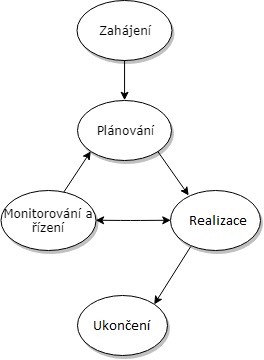
\includegraphics[scale=1.25]{Pic/planingDiagram.png}
\end{center}
\label{pic:planingDiagram}
\caption{Plánovací diagram}
\end{figure}


Projekt začíná zahájením a končí uzavřením. Fáze plánování, realizace a monitorování a řízení se mohou opakovat až do ukončení projektu. Diagram fází viz Obrázek \ref{pic:planingDiagram}. Vodopádový model má pak jednotlivé fáze za sebou tak, že přechod do další fáze je až tehdy, když je daná fáze kompletně ukončena.

\section{Softwarové chyby}
Softwarové chyba (také nazývána jako \uv{softwarový bug}) se dá definovat jako chyba, defekt, porucha či selhání v počítačovém programu nebo systému, která způsobuje vytváření nekorektních nebo neočekávaných výsledků a nebo nezamýšlené chování. 

Softwarové chyby, jsou nedílnou součástí každého softwaru. Projekt větších rozměrů bez žádné softwarové chyby je velmi vzácný, tedy se dá předpokládat, že v nějaké fázi vývoje se objeví nějaký bug. Proces hledání a řešení bugů je nazýván jako \uv{debugování} a často používá techniky nebo nástroje pro určení bugu. 

\subsection{Testování aplikací}
Testování aplikací slouží pro zamezení vydání produktu, který obsahuje chyby jakéhokoliv druhu. Testy mají vliv na kvalitu výsledného produktu, tím pádem se snaží pokrýt co nejvíce případů použití, které mohou nastat.

Samotné bugy vznikají již při realizaci daného projektu a jsou často nalezeny při testování daného řešení samotným vývojářem, nebo nástroji používanými pro překlad a vývoj. Další proces, používaný pro nalezení bugů, je takzvaný \uv{code review}, tedy revize kódu. Při tomto procesu se na cizí kód(vytvořený jiným vývojářem) podívá další vývojář a překontroluje kód, za účelem ověření funkcionality a nalezení potencionálních problémů, které původního autora kódu nemusely napadnout. 

Dalším zdrojem odhalení bugů je testování kódu. Existuje spoustu druhů technik testování. Jedním z hojně používaných druhů testů jsou takzvané jednotkové testy. Ty z pravidla píší samotní vývojáři a slouží k ověření funkcionality části kódu. Hlavním účelem těchto testů je odhalení funkční chyby v případě, že je nutné změnit část kódu. Tyto testy pak slouží pro zajištění stejné funkcionality i po změně. Bugy, které jsou nalezeny v tomto stádiu se nedostanou do žádných záznamů, jelikož jsou ihned opraveny vývojáři, kteří upravují danou část kódu.

Když je aplikace ve fázi, kdy je testovatelná, tedy je vyvinuta, lze ji nainstalovat či spustit a je přístupná, pak se obvykle spouštějí takzvané smoke testy. Smoke testy slouží k ověření, zda je aplikace vhodná k testům a obvykle se zaměřují na hlavní funkce aplikace, které nebývají často upravovány, a to pouze v jejich pozitivním průběhu. Je velmi žádoucí testy automatizovat, neboť se u nich předpokládá, že budou často spouštěny.

\subsubsection*{Systémové testy}
Zaměřují se na aplikaci jako celek v podobě, v jaké by ji měl používat zákazník. Zde se již ověřuje soulad reálného chování s chováním očekávaným, provádí se testování možných negativních průběhů, validují se výstupy a podobně.

 





TODO Pri jakzch fazich vznikaji bugy \href{https://en.wikipedia.org/wiki/Project_management}{link2} 

TODO  pridat vyznamnost bugu \href{https://www.getzephyr.com/insights/agile-strategies-managing-bug-fixes}{link3} 

TODO Moznosti zapisovani bugu - github, jira, bugzilla, redmine \href{https://en.wikipedia.org/wiki/Bug_tracking_system}{link4} 

TODO pridani vyhody trackovani- snadna detekce duplikatu, klasifikace - prideleni odpovednym oddelenim, klasifikace - nejpravdepodobnejsi pricina, prioritizace
\href{https://backlog.com/bug-tracking-guide/}{link5} 

TODO zakladni klasifikace chyb



\chapter{Klasifikační metody}








 
% 
% PRO ANGLICKOU SAZBU JE NUTNÉ ZMĚNIT
% CITAČNÍ STYL!
%
\bibliographystyle{csplainnatkiv}
{\raggedright\small
\bibliography{literatura}
}

\end{document}
